% Created 2021-01-03 Sun 20:26
% Intended LaTeX compiler: pdflatex
\documentclass[a4paper]{report}
\usepackage[utf8]{inputenc}
\usepackage[T1]{fontenc}
\usepackage{graphicx}
\usepackage{grffile}
\usepackage{longtable}
\usepackage{wrapfig}
\usepackage{rotating}
\usepackage[normalem]{ulem}
\usepackage{amsmath}
\usepackage{textcomp}
\usepackage{amssymb}
\usepackage{capt-of}
\usepackage{hyperref}
\usepackage[francais, english]{babel}
\usepackage{graphicx}
\date{\today}
\title{}
\hypersetup{
 pdfauthor={},
 pdftitle={},
 pdfkeywords={},
 pdfsubject={},
 pdfcreator={Emacs 27.1 (Org mode 9.3)}, 
 pdflang={English}}
\begin{document}

\begin{LaTex}
\begin{titlepage}
\centering
  {\scshape Hénallux\par\vspace{0.2cm} Section sécurité des systèmes\par \vspace{0.2cm}}
  \vspace{1cm}
  
\includegraphics[width=0.5\textwidth]{img/school}\par\vspace{1cm}
  {\scshape \LARGE Développement \par}
  \vspace{0.2cm}
	{\scshape \Large Implémentation d'un IDS\par}
  \vspace{3cm}
  {\Large\itshape Projet réalisé par \par\vspace{0.5cm} Mustafa-Can KUS \par Jordan DALCQ \par}
  \vfill
  \scshape Année académique 2020-2021 
  \title{Implémentation d'un IDS}
  \author{Mustafa-Can KUS Jordan DALCQ}
  \date{2020-2021}
\end{titlepage}

\pagestyle{headings}
\end{LaTex}
\tableofcontents

\part{Introduction}
\label{sec:orgae3e221}
\chapter{Contexte}
\label{sec:org4a86ad6}
Dans le cadre du cours de développement il nous a été demandé de réaliser un système de détection d'intrusion (ou IDS pour faire plus court).
Ce programme à pour but d'analyser le trafic réseau et reporter toutes activité suspectes à un administrateur système ou même un administrateur réseau
grâce à un système de log.

\chapter{Outils utilisés}
\label{sec:org9905d3c}
\section{Org mode}
\label{sec:orgf4c7e20}
Org mode est un mode majeur pour le logiciel GNU Emacs qui permet de prendre note et maintenir une "To do list" et permet aussi de planifier facilement des projets
grâce à son langage Markup (très proche du markdown). On l'a utilisé pour écrire ce rapport (ok on a un peu triché on a mit un peu de Latex pour faire joli) et aussi
pour planifier notre travail 

\begin{center}
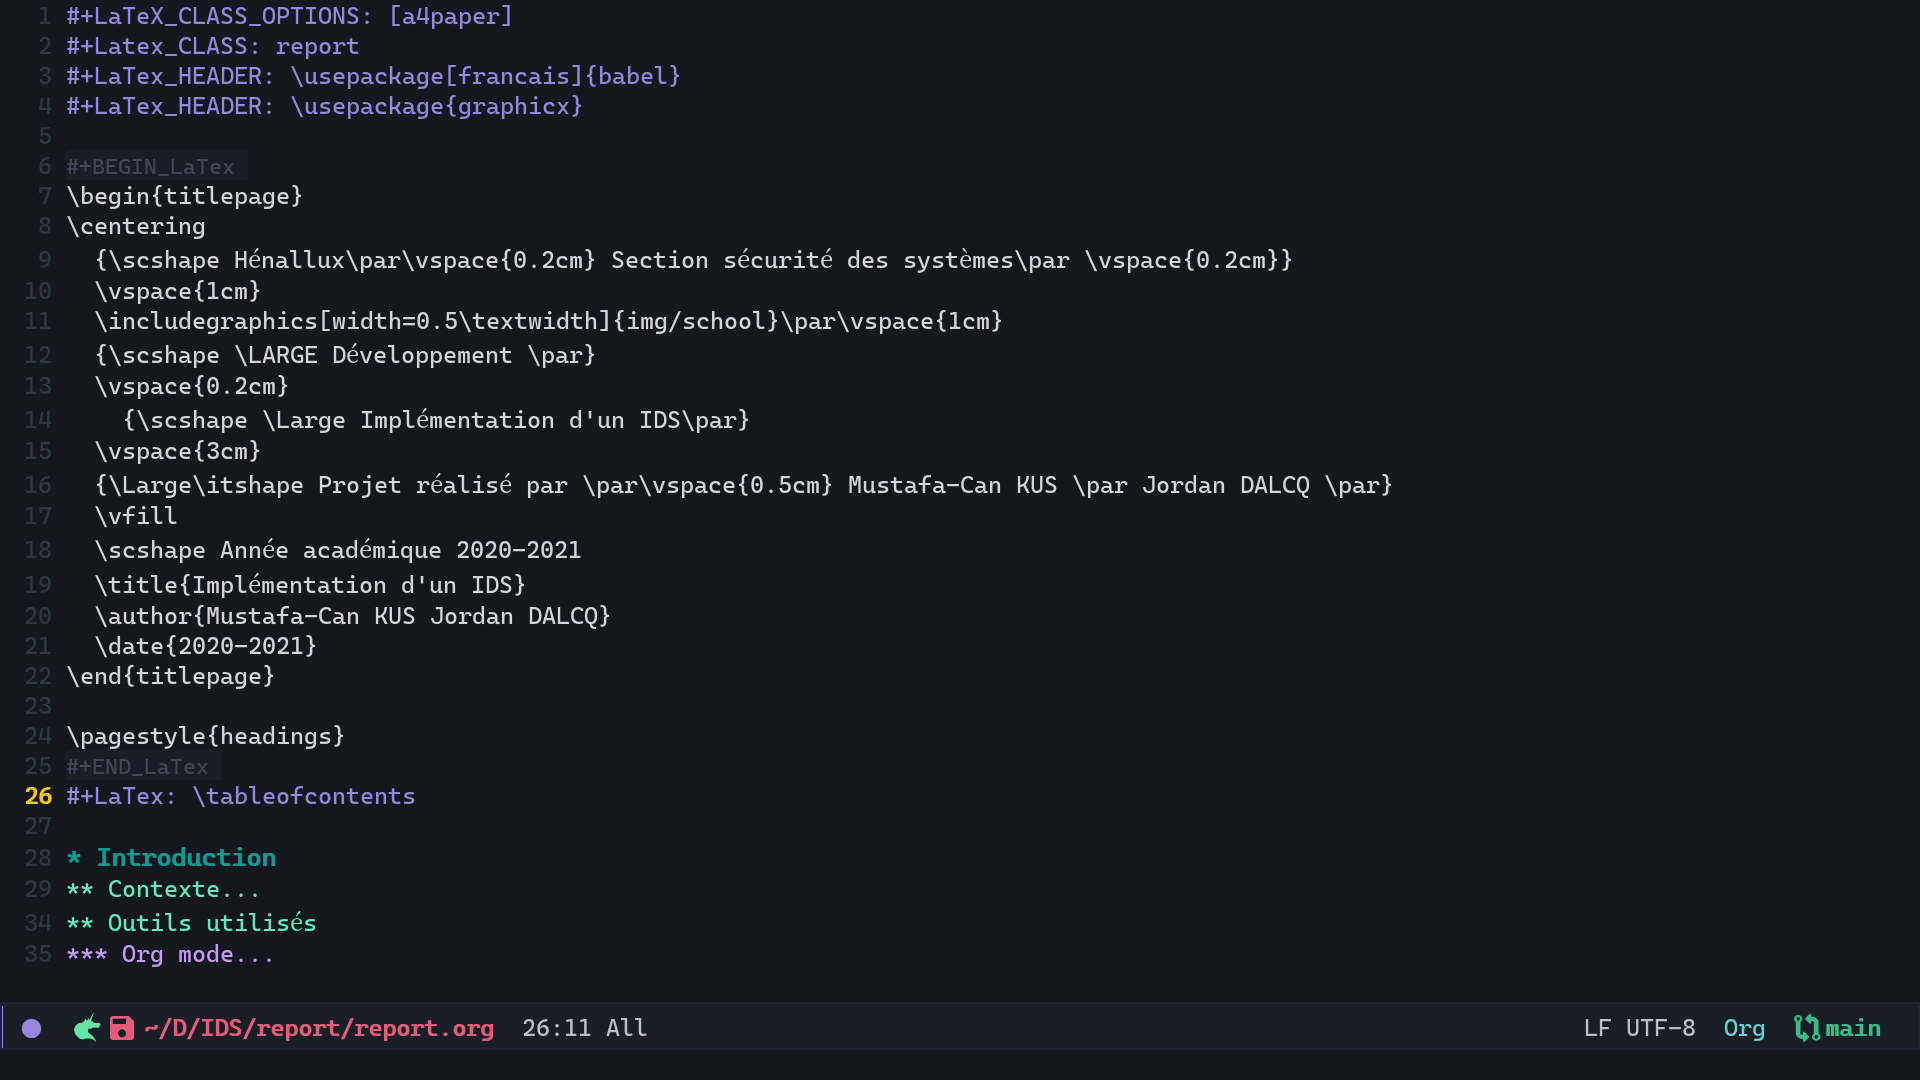
\includegraphics[width=.9\linewidth]{./img/org.png}
\end{center}
\section{Github}
\label{sec:org895be39}
Une fois notre planning fait il nous fallait une solution pour que chacun d'entre nous dispose d'une copie du code à portée de main  
et qu'on puisse tracker nos modifications, ce qui est très pratique en cas de bug, en effet il nous suffit de revenir 
quelques modifications en arrière et le problème est réglé !

Notre projet est disponible ici:
\begin{LaTex}
\begin{center}
    {\small \url{https://github.com/Les-IRaniens/IDS}}
\end{center}
\end{LaTex}
\section{GNU Makefile}
\label{sec:org6ac154f}
Comme tout bon informaticien qui se respecte, on a pas envie de taper une très longue commande composé d'une dizaine de fichiers et d'une
autres dizaine de flag à chaque fois qu'on souhaite compiler notre programme, alors on a décidé d'utiliser un makefile. 
Le makefile s'occupe de la compilation et de linker notre code automatiquement, il suffit de taper make dans le terminal et le tour est joué !
\section{Nos flags de compilations}
\label{sec:org8947535}
\begin{itemize}
\item -pednatic: nous oblige fortement à adhérer aux règles de l'ANSI C
\item -Wpednatic: nous affiche des warnings si on respecte pas la pedantique
\item -Wall: nous permet d'avoir tous les warnings sur des pratiques considérées comme questionnable
\item -Wextra: Couvre encore plus de warnings que -Wall
\item -Werror: Transforme tous les warnings en erreur (Oui on est sans pitié ici)
\item -g: Permet d'avoir les symboles de debuggage
\item -Isrc/: Permet d'inclure facilement les headers du dossier src
\item -fsanitize=undefined \& -fsanitize=undefined: Permet de tracker chaque memory leak et nous dit sur quelle ligne est le problème
\item -lpcap: Inclut la libpcap à notre projet.
\end{itemize}

\section{ArchLinux}
\label{sec:orgb12fcba}
Programmer sur Kali c'est pas top, surtout sur une VM ! Donc on a préféré utiliser ArchLinux pour le travail sur machine native.
Pourquoi cela ? Car Archlinux est une distribution polyvalante qui a TOUS les paquets qu'on désire (oui même tous les paquets de Kali).

\section{Vscodium}
\label{sec:org641df5b}
C'est Visual Studio Code - les fonctions de télémétries, c'est notre éditeur de choix, car il permet une super bonne intégration avec notre github,
nous informe de nos erreurs et des warnings potentiels grâce à l'extension C/C++.
\part{Explications du code}
\label{sec:orgba8b3a9}
Dés le départ nous avons pensé à subdiviser le code en plusieurs fichiers, cela permet de limiter le nombre de ligne de code, en effet le maximum par fichier est de 300 lignes de code, ce qui permet de trouver nos erreurs plus efficacement.

\chapter{main.c}
\label{sec:org498795a}
\section{int main (int argc, char *argv[])}
\label{sec:orgc0a11f4}
C'est un peux le chef d'orchestre de notre programme, ce fichier contient la fonction main qui donne les entrées utilisateurs au différentes fonctions grâce
aux paramètres donné au programme (argv) et vérifie que l'utilisateur démarre bien le programme avec \sudo$\backslash$.

\chapter{usage.c}
\label{sec:org9aed2c6}
\section{void show\_usage(char *exe\_path})}
\label{sec:org0f90895}
Si l'utilisateur nous donne aucun paramètre ou si il nous donne le paramètre d'aide (-h | --help)
la fonction main nous envoie sur cette fonction et nous montre un message d'utilisation. L'argument exe$\backslash$\_path} comprend le chemin de l'executable
et on récupère que le nom de l'executable (grâce à la fonction basename).

\chapter{checkuser.c}
\label{sec:orgc8e7869}
\section{bool is\_root(void)}
\label{sec:org4a218cb}
Il s'agit d'une simple vérification pour voir si on démarre bien le programme en tant qu'administrateur système.
\chapter{utils/list.c}
\label{sec:orgf61b49a}
\section{void init\_str\_list(StrList *self)}
\label{sec:orgfa3f94c}
Cette fonction est le constructeur de notre objet StrList (il s'agit d'une structure qui correspond à un tableau de string alloué de manière automatique)
Il attribue un emplacement mémoire de base.
\section{void append\_str}\_list(StrList *self, const char *str)}
\label{sec:org43b51ed}
La fonction vérifie tout d'abord si notre liste à assez de place en mémoire, si ce n'est pas le cas on lui donne plus d'emplacement mémoire
et on ajoute la chaîne de caractère donné en paramètre à la fin de la liste.
\section{StrList split\_to\_liststr(char *str, const char *del)}
\label{sec:org7924651}
Cette méthode découpe une chaîne de caractère selon un délimiteur et met chaque partie dans une liste.
\section{void free\_str\_list(StrList *self)}
\label{sec:org7cccf8f}
Cette fonction libère la mémoire occupée par une liste.
\chapter{utils/log.c}
\label{sec:org46eb15d}
\section{void log\_ids(const char *msg)}
\label{sec:org58f7673}
Cette fonction écrit dans le syslog.
\chapter{readrules.c}
\label{sec:org9176bfb}
\section{StrList read\_rules(const char *filename)}
\label{sec:org3787a2a}
C'est ici que se produit la lecture des règles (données en paramètre par l'utilisateur), le fichier est lu ligne par ligne et 
placé dans une liste de string.
\chapter{rule.c}
\label{sec:org51b8471}
\section{RuleList parse\_rule(StrList rules)}
\label{sec:org098bfed}
Voilà la fonction qui est responsable de traduire chaque règle en une structure qu'on a simplement nommé \Rule$\backslash$, qu'on place dans une liste
qu'on a nommé \RuleList$\backslash$ qui occupe un certain emplacement mémoire; la struct rule contient le protocole, l'addresse ip de source et de destination, le protocole de source et de destination. 
\section{bool is\_in\_context(Rule rule, void *packet, Protocole proto)}
\label{sec:org499a58b}
Cette fonction vérifie si le paquet correspond avec une des règles.
\section{free\_rules(RuleList *lst)}
\label{sec:org76e0eca}
cette fonction libère l'emplacement mémoire pris par les listes de règles.
\chapter{scan.c}
\label{sec:org43ece51}
\section{void scan\_network(char *interface, RuleList rules)}
\label{sec:org5dc8df8}
Cette fonction permet de préparer la libpcap et le scan du réseau.
\section{void handler(u\_char *user, const struct pcap\_pkthdr *header, const u\_char *packet)}
\label{sec:org564e8a6}
Cette fonction est le point central de notre IDS, elle capture et analyse chaque paquet qui passe par le réseau, 
elle utilise la fonction populate (présente dans le fichier populate.c) pour convertir les données binaires reçues dans le réseau
vers des structures plus simples à travailler. Si une règle correspond ; il donne un message prédéfini dans le dossier des règles au système de log de l'IDS.
\part{Critère de dépassement}
\label{sec:org8df707a}
Voici une petite liste des petits plus qu'on a ajouté au projet
\begin{itemize}
\item Utilisation des services Linux pour faire tourner l’application en tâche de fond (make install).
\item Construire une règle permettant de détecter une attaque de type XSS (simple).  Cette règle devra être utilisable dans votre IDS :
\end{itemize}
Pour cela nous avons ajouté un nouveau paramètre dans les règles nommé client-side-content, ce paramètre se comporte comme content mais s'occupe que du côté client et ignore le côté serveur.
\begin{itemize}
\item Gestion des versions (Github).
\item On a un Makefile (Ca compte comme bonus non ?).
\end{itemize}
\end{document}
